\documentclass[tikz,border=5mm]{standalone}
\usepackage{xcolor}

% Farbdefinition für die roten Elemente
\definecolor{crimsonred}{RGB}{186, 45, 63}

\begin{document}
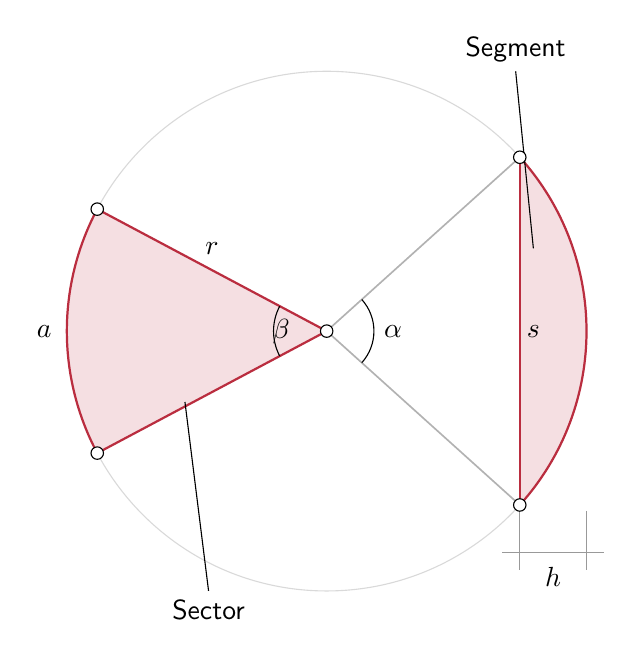
\begin{tikzpicture}[scale=1.5]
    % Parameter für den Radius
    \def\r{2.2}
    
    % 1. Hintergrund-Kreis (hellgrau und dünn)
    \draw[gray!30, thin] (0,0) circle (\r);
    
    % ==========================================
    % LINKER BEREICH: SECTOR (Winkel beta)
    % ==========================================
    % Winkel-Definition für den Sektor (symmetrisch zur Mitte)
    \def\startBeta{152}
    \def\endBeta{208}
    
    % Gefüllter und umrandeter Sektor
    \draw[crimsonred, thick, fill=crimsonred!15] (0,0) -- (\startBeta:\r) arc (\startBeta:\endBeta:\r) -- cycle;
    
    % Winkelbogen und Beschriftung für beta
    \draw[black, thin] (\startBeta:0.45) arc (\startBeta:\endBeta:0.45);
    \node[left, xshift=3pt] at (180:0.3) {$\beta$};
    
    % Beschriftung für Bogen a und Radius r
    \node[left, xshift=-2pt] at (180:\r) {$a$};
    \node[above, yshift=2pt] at (\startBeta:0.5*\r) {$r$};
    
    % Zeiger und Text für "Sector"
    \draw[black, thin] (-1.0, -2.2) -- (-1.2, -0.6);
    \node[below, font=\sffamily] at (-1.0, -2.2) {Sector};
    
    
    % ==========================================
    % RECHTER BEREICH: SEGMENT (Winkel alpha)
    % ==========================================
    % Winkel-Definition für das Segment
    \def\alphaHalf{42}
    
    % Graue Radien für den Winkel alpha
    \draw[gray!60, semithick] (0,0) -- (\alphaHalf:\r);
    \draw[gray!60, semithick] (0,0) -- (-\alphaHalf:\r);
    
    % Gefülltes Kreissegment (Fläche zwischen Sehne und Bogen)
    % HIER WAR DER FEHLER BEHOBEN: \alphaHalf statt \alphaHalfHost
    \fill[crimsonred!15] (\alphaHalf:\r) arc (\alphaHalf:-\alphaHalf:\r) -- cycle;
    
    % Rote Hervorhebung der Sehne s und des zugehörigen Bogens
    \draw[crimsonred, thick] (\alphaHalf:\r) -- (-\alphaHalf:\r);
    \draw[crimsonred, thick] (\alphaHalf:\r) arc (\alphaHalf:-\alphaHalf:\r);
    
    % Winkelbogen und Beschriftung für alpha
    \draw[black, thin] (-\alphaHalf:0.4) arc (-\alphaHalf:\alphaHalf:0.4);
    \node[right, xshift=-2pt] at (0:0.45) {$\alpha$};
    
    % Beschriftung für die Sehne s (leicht rechts von der Sehne platziert)
    \node[right, xshift=-1pt] at ({\r*cos(\alphaHalf)}, 0) {$s$};
    
    % Zeiger und Text für "Segment"
    \draw[black, thin] (1.6, 2.2) -- (1.75, 0.7);
    \node[above, font=\sffamily] at (1.6, 2.2) {Segment};
    
    % Masslinien für die Segmenthöhe h am unteren Rand
    \begin{scope}[shift={(0, {-\r*sin(\alphaHalf) - 0.25})}]
        % Vertikale Hilfslinien
        \draw[gray!80, thin] ({\r*cos(\alphaHalf)}, 0.2) -- ({\r*cos(\alphaHalf)}, -0.3);
        \draw[gray!80, thin] (\r, 0.2) -- (\r, -0.3);
        % Horizontale Masslinie mit Überstand
        \draw[gray!80, thin] ({\r*cos(\alphaHalf) - 0.15}, -0.15) -- ({\r + 0.15}, -0.15);
        % Beschriftung h
        \node[below, yshift=-2pt] at ({0.5*(\r + \r*cos(\alphaHalf))}, -0.15) {$h$};
    \end{scope}

    
    % ==========================================
    % KNOTENPUNKTE (Kleine offene Kreise)
    % ==========================================
    \filldraw[fill=white, draw=black, thin] (0,0) circle (1.5pt);
    \filldraw[fill=white, draw=black, thin] (\startBeta:\r) circle (1.5pt);
    \filldraw[fill=white, draw=black, thin] (\endBeta:\r) circle (1.5pt);
    \filldraw[fill=white, draw=black, thin] (\alphaHalf:\r) circle (1.5pt);
    \filldraw[fill=white, draw=black, thin] (-\alphaHalf:\r) circle (1.5pt);
    
\end{tikzpicture}
\end{document}
